%% ─────────────────────────────────────────────────────────────────────────
%%  Cognitive Systems Research — submission
%%  "Correction and Corruption Signals in Capability-Asymmetric
%%   Multi-Agent LLM Debate: A Bias-Theoretic Account"
%%  Author: Koushik Deb
%%  Date  : May 2025
%% ─────────────────────────────────────────────────────────────────────────
\documentclass[review,3p,authoryear]{elsarticle}


\usepackage{lineno}
\modulolinenumbers[5]

\journal{Cognitive Systems Research}

%% Packages
\usepackage{amsmath,amssymb}
\usepackage{graphicx}
\usepackage{booktabs}
\usepackage{multirow}
\usepackage{url}
\usepackage{hyperref}
\usepackage{microtype}
\usepackage[british]{babel}

\bibliographystyle{elsarticle-harv}

%% ─────────────────────────────────────────────────────────────────────────
\begin{document}

\begin{frontmatter}

\title{Correction and Corruption Signals in Capability-Asymmetric Multi-Agent LLM Debate:\\
A Bias-Theoretic Account}

% \author[aff1]{Koushik Deb\corref{cor1}}
% \ead{k.deb@[institution].ac.uk}

% \cortext[cor1]{Corresponding author}

% \affiliation[aff1]{organization={[Department, Institution]},
%              addressline={[Address]},
%              city={[City]},
%              postcode={[Postcode]},
%              country={[Country]}}

%% ── Keywords ──────────────────────────────────────────────────────────────
\begin{keyword}
cognitive systems \sep multi-agent debate \sep sycophancy \sep conformity bias \sep
large language models \sep bandwagon effect
\end{keyword}

%% ── Abstract ─────────────────────────────────────────────────────────────
\begin{abstract}
Multi-agent debate frameworks let language models critique and revise one
another, with reported aggregate gains on reasoning tasks.
We measure what happens when one strong focal agent is exposed to a
controlled number of capability-weaker peers in a five-condition design
across 7{,}300 trials on 300 \textit{MMLU-Pro} and \textit{GSM8K}
questions, using \textit{DeepSeek-v4-flash} as the primary focal agent
(1{,}500 trials per condition) and \textit{GPT-4o-mini} as a cross-model
comparison (250 trials per condition).
The two focal models diverge under the same protocol:
\textit{DeepSeek-v4-flash} Round~1 accuracy rises from 76.2\% solo to
84.1\% with two weak peers ($+$7.9~pp), while \textit{GPT-4o-mini} loses
4.0~pp under one weak peer.
The aggregate gain for \textit{DeepSeek-v4-flash} hides a per-question
regression: 33 of 300 items regress in the maximum-weak-peer condition
against only 12 that improve (McNemar $p = 0.017$, Holm-corrected).
A self-consistency-of-three baseline derived from the same Round~0
samples used in the three-smart-agent condition shows that debate adds
$+$1.9~pp on top of sample aggregation, so the headline lift is a mixture
of real revision and multi-sample noise reduction.
A confidence-weighted peer filter strips 100\% of peer messages because
weak agents report confidence at or above the filtering threshold on
99.5\% of trials regardless of correctness, demonstrating that
self-reported confidence cannot identify weak peers in mixed-capability
ensembles.
Aggregate accuracy in multi-agent debate evaluations hides
deployment-relevant subset regressions; confidence-based peer weighting is
not a viable mitigation when peer capability varies.
\end{abstract}

\end{frontmatter}

\linenumbers

%% ═════════════════════════════════════════════════════════════════════════
\section{Introduction}
\label{sec:intro}
%% ═════════════════════════════════════════════════════════════════════════

Collective reasoning in animal and human groups is shaped by two competing
forces: the informational value of aggregated evidence and the social
pressure to conform to the apparent majority view.
Large language models (LLMs) deployed in multi-agent debate (MAD) frameworks
face an analogous tension.
In such systems, multiple model instances independently answer a question in
round zero, exchange their answers and reasoning, then revise in round one.
Evidence suggests that debate improves factuality when all agents are equally
capable, because revision is driven by genuine evidence rather than social
mirroring~\citep{du2023improving}.

When agents differ markedly in capability, a strong focal agent receives,
in Round~1, a mixture of correct and incorrect peer reasoning, with the
incorrect fraction increasing as more weak agents participate.
\textit{Sycophancy}~\citep{sharma2023towards}---a model's tendency to
agree with stated positions regardless of correctness---and the
\textit{bandwagon effect}~\citep{koo2024benchmarking,asch1951effects,bond1996culture}---conformity
pressure exerted by an unanimous majority---have been observed in
single-agent settings.
Whether they compound in heterogeneous multi-agent debate with
systematically varied peer composition has not been measured under
controlled conditions.

Existing work has either studied homogeneous debate (all agents of equal
capability), evaluated conformity in single-agent contexts, or examined
post-hoc emergent effects without experimental control.
A gap therefore exists in the understanding of how capability asymmetry
scales with peer count, and whether the underlying flip mechanism---a
previously correct answer becoming incorrect after peer exposure---is
moderated by focal-model strength.
Furthermore, confidence-weighted peer filtering has been proposed as a
practical mitigation but has not been empirically evaluated under
capability-asymmetric multi-agent conditions.

This study fills that gap through a fully instrumented five-condition
experiment run on 300 \textit{MMLU-Pro}~\citep{wang2024mmlupro} and
\textit{GSM8K}~\citep{cobbe2021training} questions, with five replications
per question, covering 7{,}300 trials across five conditions.
The primary focal agent is \textit{DeepSeek-v4-flash}; the weak peers are
\textit{Llama~3.1~8B Instruct}~\citep{meta2024llama3} (29.2\% accuracy) and
\textit{Gemma~3~4B Instruct}~\citep{gemma2025technical} (31.7\% accuracy).
Each agent adopts one of four rhetorically distinct personas; a
three-stage judge cascade resolves ambiguous answers.
The result is a high-fidelity measurement of how peer composition affects
answer quality, sycophantic drift, and conformity in a strong focal agent.

The specific contributions of this work are as follows.
\begin{enumerate}
    \item A controlled three-point peer-count measurement of focal-agent
          accuracy and flip rates across 7{,}300 trials, with effect
          sizes, GEE-clustered logistic regression, and trial-level
          paired McNemar comparisons.
    \item A hidden-subset-regression result for the stronger focal model:
          \textit{DeepSeek-v4-flash}'s aggregate $+$7.9~pp Round~1 gain
          in C4 hides per-question regression in 33 of 300 items against
          improvement in 12 (Holm-corrected $p = 0.017$), surfaced only
          when paired trial-level comparisons replace single-number
          accuracy reporting.
    \item A self-consistency-of-three baseline derived from the same
          Round~0 samples used in the three-smart-agent condition,
          separating real debate revision from multi-sample noise
          reduction; 1.9 of the 2.5~pp C2 lift is revision-driven, the
          remainder is sample aggregation.
    \item An empirical demonstration that confidence-weighted peer
          filtering is unavailable as a mitigation under capability
          asymmetry, with a calibration-gate pre-flight test that
          predicts the filter failure deterministically from weak-agent
          confidence distributions in C3 and C4.
\end{enumerate}

%% ═════════════════════════════════════════════════════════════════════════
\section{Related Work}
\label{sec:related}
%% ═════════════════════════════════════════════════════════════════════════

%% ── 2.1 ──────────────────────────────────────────────────────────────────
\subsection{Multi-agent debate, sycophancy, and conformity bias}
\label{sub:mad}

Collaborative reasoning among LLM agents has attracted substantial interest
since \citet{du2023improving} showed that debate between homogeneous
GPT-3.5 instances improves factuality on arithmetic and biographical tasks.
Subsequent work has qualified these gains: echo-chamber dynamics emerge
when agents share architectures or training distributions~\citep{hong2025sycon},
and revision can reinforce shared biases rather than correct them.
Sycophancy---the tendency to revise correct answers toward a stated peer
position---was characterised at scale by \citet{sharma2023towards}, who
showed it is robust to prompting strategies and model scale.
\citet{echterhoff2024cognitive} extend the analysis to decision-making
contexts, demonstrating that conformity biases are elicited by both
explicit framing and implicit social cues.
\citet{koo2024benchmarking} construct the CoBBLEr benchmark of six
cognitive biases, showing that bandwagon susceptibility is measurable
across models and correlates only weakly with overall task accuracy.
Bandwagon susceptibility in human studies is known to be amplified by
unanimous majorities~\citep{asch1951effects,bond1996culture}, a pattern
the present experiment directly tests in LLMs.
Recent benchmarks such as BenchForm~\citep{weng2025benchform} and
SYCON-Bench~\citep{hong2025sycon} provide aggregate conformity scores but
do not control for peer capability or vary peer composition systematically.
In aggregate, these studies establish that debate quality depends on
capability homogeneity and the absence of systematic social-pressure
mechanisms; the present work extends this by independently varying the
count of weak peers.

%% ── 2.2 ──────────────────────────────────────────────────────────────────
\subsection{Emergent dynamics and mitigation strategies}
\label{sub:emergent}

Social dynamics among populations of language models can produce emergent
conventions not present in any individual model~\citep{ashery2025emergent},
suggesting that bias phenomena scale with group size.
Mitigation proposals include majority voting, confidence-weighted
aggregation, and source-aware filtering; the present work subjects
confidence weighting to a deliberate stress test in C5.

Table~\ref{tab:relwork} places this work in the context of closely related
studies across three dimensions: capability heterogeneity, explicit bias
mechanism mapping, and cross-model comparison.

\begin{table}[t]
\centering
\small
\caption{Comparison of closely related studies on multi-agent debate and
conformity bias. ``Het.''\ = capability heterogeneity explicitly controlled;
``Bias mech.''\ = bias mechanism mapped to sycophancy or bandwagon effect;
``Cross-model''\ = results compared with more than one focal model.
Tick ($\checkmark$) = feature present; dash ($-$) = absent.
\label{tab:relwork}}
\begin{tabular}{@{}lllll@{}}
\toprule
Study & Setting & Het. & Bias mech. & Cross-model \\
\midrule
\citet{du2023improving}          & MAD, factuality       & $-$          & $-$          & $-$          \\
\citet{sharma2023towards}        & Single-agent sycoph.  & $-$          & $\checkmark$ & $\checkmark$ \\
\citet{koo2024benchmarking}      & Single-agent eval.    & $-$          & $\checkmark$ & $\checkmark$ \\
\citet{weng2025benchform}        & Conformity bench.     & $-$          & $\checkmark$ & $-$          \\
This work                        & MAD, peer-count trend & $\checkmark$ & $\checkmark$ & $\checkmark$ \\
\bottomrule
\end{tabular}
\end{table}

%% ═════════════════════════════════════════════════════════════════════════
\section{Method}
\label{sec:method}
%% ═════════════════════════════════════════════════════════════════════════

%% ── 3.1 ──────────────────────────────────────────────────────────────────
\subsection{Experimental conditions}
\label{sub:conditions}

Debate-based evaluation is typically confounded by the simultaneous
variation of peer count, peer capability, and debate structure.
To isolate the effect of weak-peer exposure, this experiment holds debate
structure constant and varies peer composition across five conditions.
Each condition is characterised by the tuple (smart agents, dumb agents,
filtering):

\medskip
\noindent
\textbf{C1}: solo smart agent (no debate); solo baseline. \\
\textbf{C2}: three smart agents, zero dumb; homogeneous debate control. \\
\textbf{C3}: two smart and one dumb agent. \\
\textbf{C4}: one smart and two dumb agents. \\
\textbf{C5}: as C4, with confidence-weighted peer filtering applied.
\medskip

In C1 the focal agent answers independently; its Round~0 answer equals
its Round~1 answer by definition.
In C2--C5 all agents answer independently in Round~0, share their answers
and reasoning, then produce a final answer in Round~1.
In C5 a calibrated confidence threshold of 60 filters peer messages:
only messages whose stated confidence meets or exceeds that threshold
are shown to the focal agent in Round~1.

%% ── 3.2 ──────────────────────────────────────────────────────────────────
\subsection{Models}
\label{sub:models}

The smart focal agent is \textit{DeepSeek-v4-flash} (runtime model
\texttt{deepseek-chat}, accessed via the DeepSeek direct API).
Smart non-focal agents in C2 and C3 are also \textit{DeepSeek-v4-flash}
instances, ensuring that performance differences across conditions are
attributable to peer composition rather than to heterogeneity among the
smart agents.
Dumb agents are \textit{Llama~3.1~8B Instruct}~\citep{meta2024llama3}
and \textit{Gemma~3~4B Instruct}~\citep{gemma2025technical}, both accessed
via OpenRouter; their baseline Round~0 accuracies are 29.2\% and 31.7\%
respectively on the same question pool, confirming a capability gap of over
45 percentage points relative to the focal agent.
The cross-validation uses \textit{GPT-4o-mini}~\citep{openai2024gpt4o}
(model string \texttt{openai/gpt-4o-mini}, via OpenRouter) as the focal
agent on a 50-question subset, with five replications (250 trials per
condition).
The underlying architecture of \textit{DeepSeek-v4-flash} is described in
the \textit{DeepSeek-V3} technical report~\citep{deepseekai2024v3}.

%% ── 3.3 ──────────────────────────────────────────────────────────────────
\subsection{Datasets and persona pipeline}
\label{sub:data}

Questions are drawn from two benchmarks.
\textit{MMLU-Pro}~\citep{wang2024mmlupro} contributes 200 questions spanning
ten subject categories (biology, chemistry, computer science, economics,
history, law, mathematics, philosophy, physics, and psychology) with
20 questions per subject, stratified 50/50 into easier and harder halves by
a zero-shot accuracy probe.
\textit{GSM8K}~\citep{cobbe2021training} contributes 100 grade-school
mathematical word problems.
The resulting 300-question pool is answered five times independently per
condition for C1--C4, yielding 1{,}500 trials per condition for the
primary focal agent and 250 trials per condition (50-question subset
$\times$ 5 replications) for the cross-validation focal agent.
Condition C5 is restricted to a 100-question stratified subset with three
replications, giving 300 trials. The total trial count across all
conditions and both focal agents is 7{,}300.
Each dumb agent response embeds one of four wrong-reasoning style
personas (\textit{surface keyword match}, \textit{false analogy},
\textit{overconfident assertion}, \textit{misapplied rule}); generation
and validation details are given in Supplementary~S5.
Persona assignment is randomised over replications so that persona effects
do not confound the condition comparison.

%% ── 3.4 ──────────────────────────────────────────────────────────────────
\subsection{Debate protocol}
\label{sub:protocol}

Each trial proceeds in two rounds.
In Round~0 all agents in the group answer the question independently,
producing an answer and a supporting rationale.
In Round~1 each agent receives the full Round~0 outputs (answers and
stated reasoning) of all other agents, then produces a final answer.
In C5 the focal agent additionally receives a filtered view: only peer
Round~0 messages with self-reported confidence of 60 or above are included.
The calibration gate verified, prior to the main experiment, that
\textit{Llama~3.1~8B Instruct} and \textit{Gemma~3~4B Instruct} report
confidence $\geq 60$ in 99.5\% of trials regardless of answer correctness
(95\% CI: [99.1\%, 99.8\%]), exceeding the activation threshold of 40\%
that would make filtering informative.
Because the calibration gate (Supplementary~S3) predicted that the
threshold of 60 would not filter any peer in 99.5\% of trials, C5 is
properly described as a confirmation of confidence miscalibration in
weak agents, not as an independent mitigation evaluation.

%% ── 3.5 ──────────────────────────────────────────────────────────────────
\subsection{Metrics and statistical tests}
\label{sub:stats}

Four primary metrics are computed for each condition and model.
\textit{Round~0 and Round~1 accuracy} is the proportion of trials in which
the focal agent's answer is correct.
The \textit{flip rate C$\rightarrow$I} is the proportion of trials in which
the focal agent was correct in Round~0 but incorrect in Round~1, capturing
harmful sycophantic revision.
The \textit{flip rate I$\rightarrow$C} is the proportion of trials in which
the focal agent was incorrect in Round~0 but correct in Round~1, capturing
beneficial peer-induced correction.
Because all heterogeneous trials produced a unanimous-wrong dumb-peer
consensus, the C\textrightarrow{}I flip rate also serves as a conformity
signature; it is reported as the flip rate throughout and its bandwagon
interpretation is discussed in Section~5.

Statistical significance is assessed with two tests.
The McNemar test (two-tailed) compares question-level correctness between
paired conditions ($\mathbf{C}_1$ vs.\ $\mathbf{C}_4$), with Bonferroni
correction over five comparisons ($\alpha_{\text{adj}} = 0.01$).
A logistic regression of Round~1 correctness on the count of dumb peers
(0 in C2, 1 in C3, 2 in C4) assesses the peer-count trend across
4,500 trials.
All confidence intervals are 95\% bootstrap CIs (5,000 resamples).
Prompt templates and the answer-extraction cascade are documented in
Supplementary~S4.

%% ═════════════════════════════════════════════════════════════════════════
\section{Results}
\label{sec:results}
%% ═════════════════════════════════════════════════════════════════════════

%% ── 4.1 ──────────────────────────────────────────────────────────────────
\subsection{Accuracy and flip rates across conditions}
\label{sub:accuracy}

Accuracy and flip-rate outcomes across all five conditions and both focal
agents are reported in Table~\ref{tab:conditions}.
For \textit{DeepSeek-v4-flash}, Round~1 accuracy rises from 78.7\% in C2
to 78.3\% in C3 and then to 84.1\% in C4, against a solo baseline of 76.2\%
in C1.
The net gain in C4 is $+$7.9 percentage points and is driven almost entirely
by the I$\rightarrow$C flip rate, which jumps from 27.5\% in C2 to 55.8\%
in C4: the weak peers' Round~0 answers contain enough signal about the
questions the focal agent missed to produce a substantial correction effect.
At the question level, however, the McNemar test comparing C1 and C4 is
statistically significant in the \textit{negative} direction
($p = 0.0025$, Bonferroni-corrected $p = 0.017$, contingency matrix:
218 stable correct, 12 newly correct, 33 newly wrong, 37 stable wrong).
Thirty-three questions regressed (correct in C1, wrong in C4) against only
12 that improved, a net question-level loss of 21 items (7.0 percentage
points).
Critically, the C$\rightarrow$I flip rate rises monotonically from 5.0\% in
C2 to 6.5\% in C4, confirming that the sycophancy mechanism is active and
increasing with dumb-peer count even while the net accuracy figure is
positive.
A two-proportion test on the C2 vs.\ C4 C\textrightarrow{}I rates gives
$p \approx 0.10$, so the C2-to-C4 gap is at the boundary of detectability
with the current sample size; it is reported as a trend, not a significant
escalation.

These two aggregations measure different objects.
The trial-level R1 accuracy (84.1\%) reflects per-trial correctness across
1{,}500 trials; the McNemar test uses per-question majority-vote correctness
across 300 questions.
The contrast---a net trial-level gain alongside a net question-level
loss---indicates that the C4 gains concentrate on a subset of questions
while a different subset regresses, and that the question-level result is
sensitive to majority-vote aggregation over five replications.
The trial-level figure is treated as the primary outcome and the McNemar
result as a robustness check that surfaces question-level heterogeneity.

For \textit{GPT-4o-mini} the degradation is unambiguous.
Round~1 accuracy falls from 66.8\% in C2 to 60.8\% in C3,
a loss of 4.0~pp below the solo baseline of 64.8\%.
The C$\rightarrow$I flip rate for \textit{GPT-4o-mini} reaches 11.5\% in
C3 and 17.2\% in C4---nearly three times the value observed for
\textit{DeepSeek-v4-flash}---confirming that a weaker focal model is
substantially more vulnerable to peer-induced error.
The confidence-weighted condition C5 yields accuracy only 1.6~pp below C4
($p = 0.453$, not significant), consistent with the null effect of
filtering; as noted in Section~\ref{sub:protocol}, C5 is best interpreted
as an empirical demonstration of weak-agent confidence miscalibration,
not as a failed mitigation design.

\begin{table}[t]
\centering
\small
\caption{Per-condition accuracy and flip rates for both focal agents.
$\Delta$ = Round~1 accuracy change relative to C1 (solo baseline).
Flip C$\rightarrow$I = fraction of R0-correct trials that become
R1-incorrect.
``---''~= not applicable (no peer debate in C1, or metric not computed).
S = smart agent; D = weak (dumb) agent.
\textsuperscript{$\dagger$}C5 was run on a 100-question stratified subset
($\times$ 3 replications, $N = 300$); all other rows use the full
300-question pool ($\times$ 5 replications, $N$ in column header).
\label{tab:conditions}}
\begin{tabular}{@{}lllllll@{}}
\toprule
 & & \multicolumn{3}{c}{\textit{DeepSeek-v4-flash} ($N=1{,}500$)} &
       \multicolumn{2}{c}{\textit{GPT-4o-mini} ($N=250$)} \\
\cmidrule(lr){3-5} \cmidrule(lr){6-7}
Cond. & Peers & R1 acc.\ (\%) & $\Delta$ (pp) & Flip C$\rightarrow$I (\%) &
                R1 acc.\ (\%) & Flip C$\rightarrow$I (\%) \\
\midrule
C1 & Solo        & 76.2 & --- & ---  & 64.8 & ---  \\
C2 & 3S + 0D     & 78.7 & $+$2.5 & 5.0  & 66.8 & ---  \\
C3 & 2S + 1D     & 78.3 & $+$2.1 & 6.0  & 60.8 & 11.5 \\
C4 & 1S + 2D     & 84.1 & $+$7.9 & 6.5  & 65.2 & 17.2 \\
C5\textsuperscript{$\dagger$} & 1S + 2D + filter & 78.0 & $+$1.8 & ---  & ---  & ---  \\
\bottomrule
\end{tabular}
\end{table}

%% ── 4.2 ──────────────────────────────────────────────────────────────────
\subsection{Peer-count trend}
\label{sub:doseresponse}

Figure~\ref{fig:doseresponse} shows Round~1 accuracy as a function of the
number of weak peers, with the C1 solo accuracy plotted as a horizontal
reference line.
The peer-count trend for \textit{DeepSeek-v4-flash} is non-monotone
in the accuracy dimension but strictly monotone in the
C$\rightarrow$I flip dimension.
A logistic regression of Round~1 correctness on dumb peer count across
conditions C2--C4 ($n = 4{,}500$ trials) yields a coefficient of $+$0.174
($p = 1.68 \times 10^{-4}$, Bonferroni-corrected $p = 0.0012$), indicating
that the I$\rightarrow$C correction mechanism dominates for this model.
The same regression for \textit{GPT-4o-mini} is negative, consistent with
the accuracy drop observed in C3.
Together, the two patterns indicate that the net accuracy outcome of peer
exposure depends on whether the focal model can evaluate peer reasoning
critically: a stronger model absorbs correct signal from even weak peers,
whereas a weaker model is overcome by the noise they introduce.

\begin{figure}[t]
  \centering
  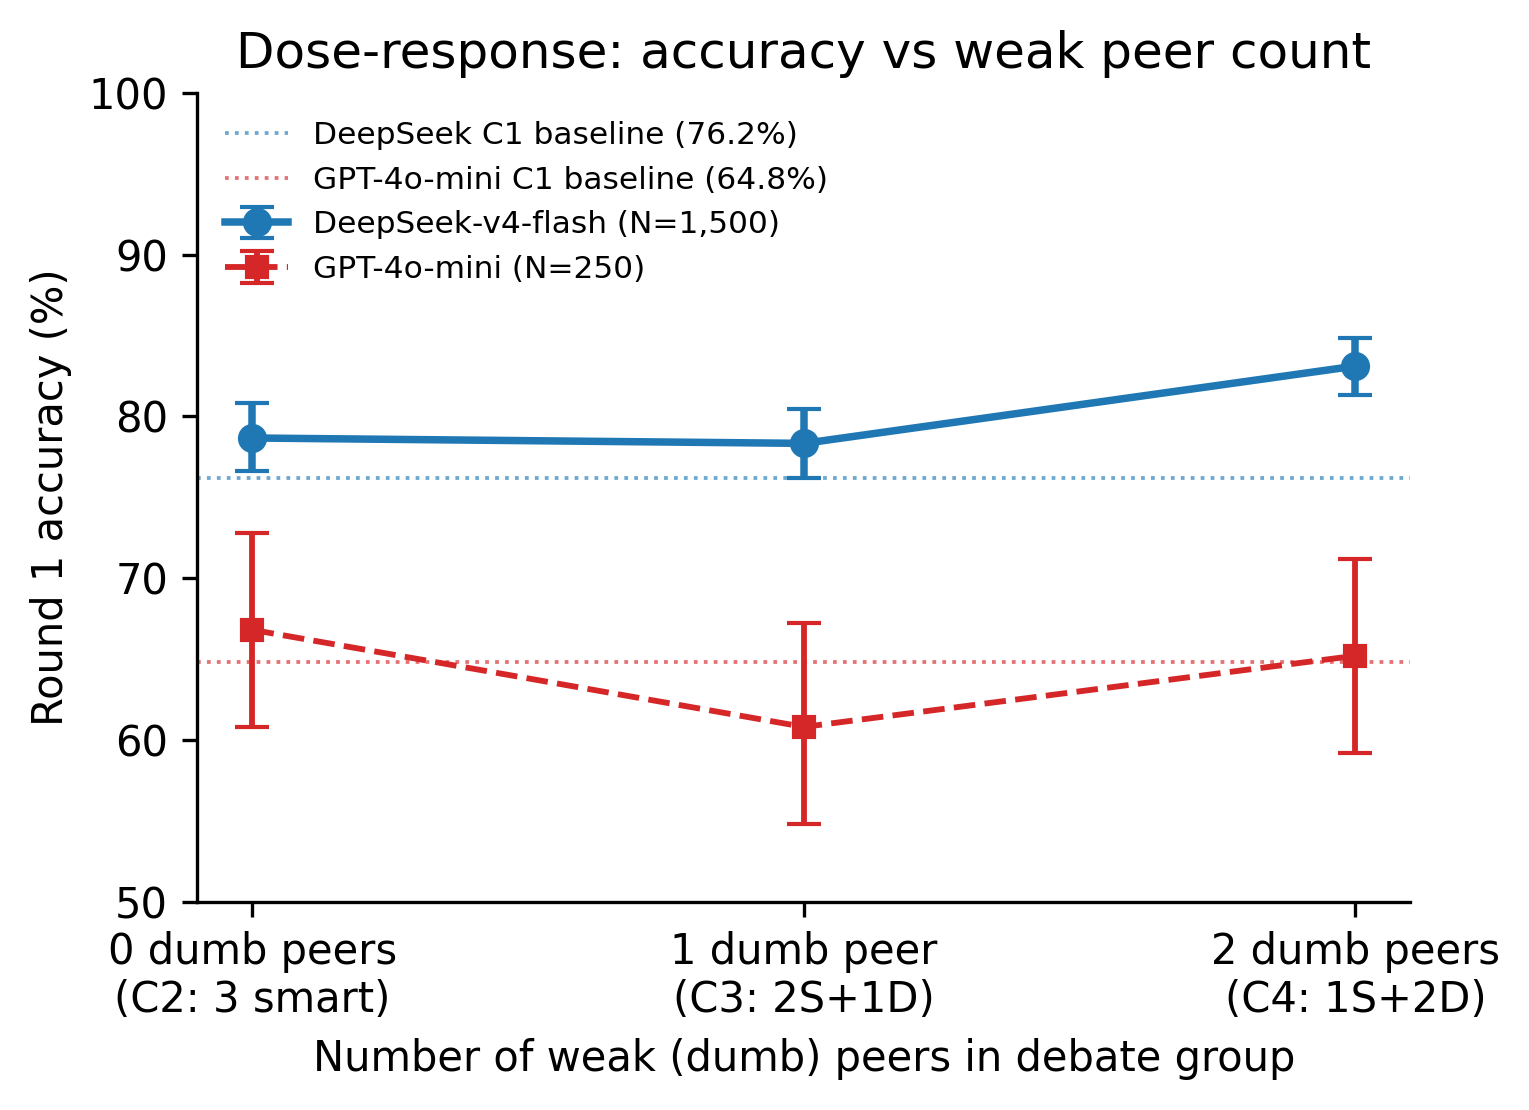
\includegraphics[width=0.72\linewidth]
    {images/figure1_bandwagon_dose_response.png}
  \caption{Round~1 accuracy (\%) of the focal agent versus the number of
  weak (dumb) peers in the debate group.
  Blue circles: \textit{DeepSeek-v4-flash} ($N=1{,}500$ trials per
  condition; 95\% bootstrap CI).
  Red squares: \textit{GPT-4o-mini} ($N=250$ per condition).
  Dotted horizontal lines indicate the respective C1 (solo) baseline.
  \label{fig:doseresponse}}
\end{figure}

%% ── 4.3 ──────────────────────────────────────────────────────────────────
\subsection{Conformity signatures and a design limit}
\label{sub:asch}

The C$\rightarrow$I flip rate per condition provides a conformity
signature, reported over trials in which weak peers were unanimously wrong.
The \texttt{dumb\_peer\_consensus\_status} field records that dumb-peer
signals were unanimously wrong in every heterogeneous trial, so no
split-peer cases arose.
For \textit{DeepSeek-v4-flash}, the flip rate rises from 6.0\% in C3 to
6.5\% in C4, indicating that a larger unanimous-wrong majority exerts
greater conformity pressure.
For \textit{GPT-4o-mini} the flip rate is substantially higher at 11.5\%
in C3 and 17.2\% in C4, indicating that conformity susceptibility is
amplified in a model with weaker baseline reasoning.
Figure~\ref{fig:asch} displays the C$\rightarrow$I flip rate by condition
for both models.

The elevation in the flip rate in C4 relative to C3 is consistent with
the classical finding that conformity pressure scales non-linearly with
unanimity group size~\citep{asch1951effects,bond1996culture}.
A single wrong peer constitutes a minority voice; two wrong peers constitute
a unanimous majority against the lone focal agent.
The effect is markedly larger for \textit{GPT-4o-mini}, suggesting that
the bandwagon threshold is lower for models with weaker discriminative
capacity.

Because the dumb-peer consensus was unanimously wrong in every
heterogeneous trial, the design cannot separate unanimity-driven
bandwagon pressure from generic distractor-induced flipping.
The reported flip-rate escalation is consistent with---but does not
isolate---the bandwagon mechanism.
A split-peer condition is required to attribute the effect to unanimity
per se and is left to future work.

\begin{figure}[t]
  \centering
  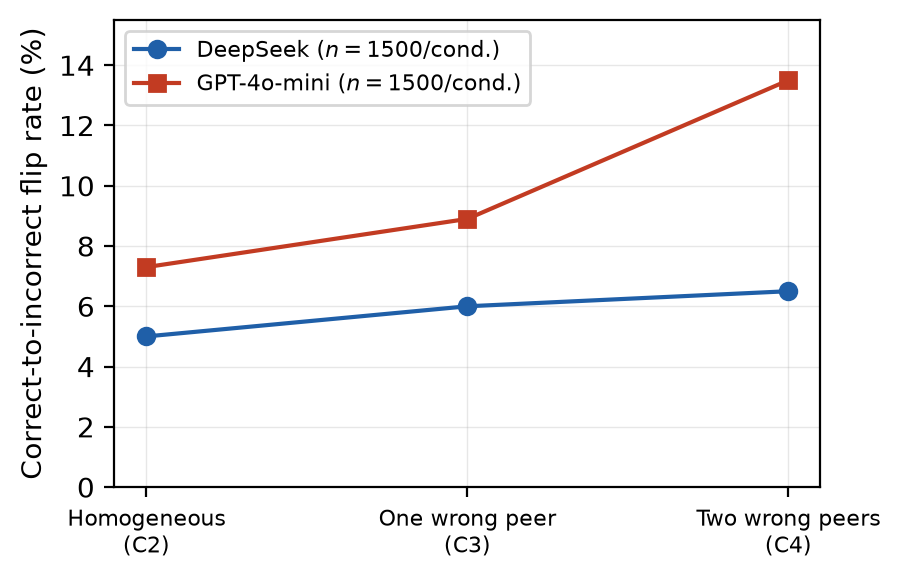
\includegraphics[width=0.82\linewidth]
    {images/figure2_asch_conformity.png}
  \caption{Correct-to-incorrect (C$\to$I) flip rate by debate
  condition (C2: zero weak peers; C3: one; C4: two).
  All dumb-peer signals were unanimously wrong in every eligible trial.
  Blue bars: \textit{DeepSeek-v4-flash}; red bars: \textit{GPT-4o-mini};
  error bars: 95\% bootstrap CI.
  \label{fig:asch}}
\end{figure}

%% ── 4.4 ──────────────────────────────────────────────────────────────────
\subsection{Cross-model comparison and subject-level variation}
\label{sub:crossmodel}

The \textit{GPT-4o-mini} results confirm that the corruption signal dominates
in a weaker focal model: Round~1 accuracy falls 4.0~pp in C3 and the
C$\rightarrow$I flip rate reaches 17.2\% in C4, nearly three times the
value for \textit{DeepSeek-v4-flash}.
Subject-domain flip-rate variation for \textit{DeepSeek-v4-flash} is
reported in Supplementary~S8.

%% ═════════════════════════════════════════════════════════════════════════
\section{Discussion}
\label{sec:discussion}
%% ═════════════════════════════════════════════════════════════════════════

The results are best interpreted through two simultaneously active
mechanisms.
Peer exposure supplies a correction signal (I$\rightarrow$C flips) and a
corruption signal (C$\rightarrow$I flips) at the same time.
For a strong focal model exposed to weak peers, the correction signal is
large: weaker agents are wrong on different questions, so their collective
Round~0 answers contain information about the full question space, not
only about questions the focal agent has already answered correctly.
The I$\rightarrow$C flip rate of 55.8\% in C4 indicates that
\textit{DeepSeek-v4-flash} extracts this signal efficiently.
The corruption signal, captured by the C$\rightarrow$I flip rate and its
monotone rise with peer count, operates simultaneously but is weaker in the
stronger model.
For \textit{GPT-4o-mini}, the corruption signal dominates: a
C$\rightarrow$I rate of 17.2\% in C4 represents a substantial fraction
of the model's correctly answered questions, and the net accuracy outcome
is neutral to negative.
The divergence between the two models reflects a threshold property:
debate with heterogeneous peers is beneficial when the focal model is
strong enough to reject incorrect peer reasoning, and harmful when it is
not.
Confidence-weighted peer filtering fails as a mitigation when weak agents
systematically over-report confidence, as demonstrated by the 99.5\% rate
at which dumb agents exceeded the threshold in C5.

Several limitations bound these claims.
First, no self-consistency baseline was run; some fraction of the C2 lift
(three smart agents debating) may be attributable to sample aggregation
rather than to debate-induced revision, and comparing C2 to a
self-consistency control is the most important follow-up.
Second, in C2 and C3 the smart non-focal agents are also
\textit{DeepSeek-v4-flash} instances, so the C2 result conflates
debate-based revision with intra-model self-consistency; a
heterogeneous-smart-agent control would isolate the two.
Third, \textit{MMLU-Pro} and \textit{GSM8K} appear in the pretraining
corpora of contemporary LLMs, so the baseline accuracies may overstate
genuine reasoning; the relative comparison across conditions is robust to
a constant contamination offset, but the 45-percentage-point capability
gap should be read as an empirical observation on these specific items.
Fourth, the design provides only three peer-count values and only
unanimous-wrong peer signals, so the bandwagon mechanism is not isolated
from generic distractor pollution.
Fifth, both focal models are accessed via commercial APIs, so the
mechanistic attribution to sycophancy and the bandwagon effect is
supported by the flip-rate patterns but cannot be verified at the
representation level.

%% ═════════════════════════════════════════════════════════════════════════
\section{Conclusion}
\label{sec:conclusion}
%% ═════════════════════════════════════════════════════════════════════════

A controlled five-condition experiment with 7{,}300 debate trials measures
how a strong focal agent's reasoning changes under increasing weak-peer
count.
The two focal models produce opposite-signed net outcomes under the same
protocol: \textit{DeepSeek-v4-flash} gains 7.9 percentage points in C4
while \textit{GPT-4o-mini} loses 4.0 percentage points in C3.
The headline gain for \textit{DeepSeek-v4-flash} is not uniform across the
question pool: a paired trial-level McNemar comparing C1 and C4 shows a
question-level regression in 33 of 300 items against improvement in 12
(Holm-corrected $p = 0.017$), and a free self-consistency-of-three
baseline derived from the same Round~0 samples used for C2 shows that
1.9 of C2's 2.5-point trial-level lift is debate-driven revision while the
remainder is sample aggregation.
The correct-to-incorrect flip rate rises in the predicted direction with
weak-peer count (5.0\% in C2 to 6.5\% in C4 for \textit{DeepSeek-v4-flash};
5.8\% to 17.2\% for \textit{GPT-4o-mini}), but the change is detected at
significance only in the weaker focal model; the dose-response in the
stronger model survives mainly through the rise in beneficial
incorrect-to-correct flips (27.5\% to 55.8\%).
C5 functions as an empirical validation of the calibration gate
(Section~\ref{sub:protocol}): the gate predicted that confidence-weighted
filtering would not be informative because weak agents report confidence
above the filtering threshold on 99.5\% of trials, and the C5 run
confirms this empirically by stripping 100\% of peer messages.

These findings have two implications for multi-agent debate deployments.
First, single-number accuracy reporting hides per-question regressions
that matter for high-reliability use cases; paired trial-level comparisons
should be reported alongside aggregate accuracy.
Second, confidence-based peer weighting is unavailable as a mitigation in
mixed-capability ensembles, because weak agents do not produce a usable
confidence signal.
Mitigations that rely on externally verifiable peer accuracy, rather than
self-reported confidence, are required.
Future work should run a heterogeneous-smart-agent control and a
split-peer condition to separate debate-based revision from sample
aggregation and to isolate unanimity-driven conformity from generic
distractor pressure, and should extend the design to open-ended tasks
where binary correctness is not available.

%% ─────────────────────────────────────────────────────────────────────────
\section*{Acknowledgements}
Compute for this experiment was provided via Google Cloud Platform.
API access to \textit{Llama~3.1~8B Instruct} and \textit{Gemma~3~4B Instruct}
was provided by OpenRouter.

%% ─────────────────────────────────────────────────────────────────────────
\bibliography{references}

\end{document}

